\documentclass[tikz,border=10pt]{standalone}
\usepackage{tikz}
\usetikzlibrary{3d, calc, arrows.meta, positioning}

\begin{document}
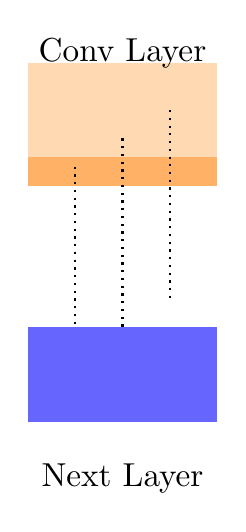
\begin{tikzpicture}[scale=1.2, transform shape]

% --- Layer A (upper block)
\coordinate (A1) at (0, 0);
\coordinate (A2) at (2, 0);
\coordinate (A3) at (2, 1);
\coordinate (A4) at (0, 1);

\coordinate (Ashadow) at (0.4, -0.3);
\def\depth{0.3}
\coordinate (Az) at (0, \depth);

% Draw Layer A front
\fill[orange!60] (A1) -- (A2) -- (A3) -- (A4) -- cycle;

% Draw Layer A top
\fill[orange!30] 
    ($(A1)+(0,\depth)$) -- ($(A2)+(0,\depth)$) -- ($(A3)+(0,\depth)$) -- ($(A4)+(0,\depth)$) -- cycle;

% Dotted projections downward
\draw[dotted, thick] ($(A1)+(1,0.5)$) -- ++(0,-2);
\draw[dotted, thick] ($(A1)+(0.5,0.2)$) -- ++(0,-2);
\draw[dotted, thick] ($(A1)+(1.5,0.8)$) -- ++(0,-2);

% --- Layer B (below)
\begin{scope}[yshift=-2.5cm]
\coordinate (B1) at (0, 0);
\coordinate (B2) at (2, 0);
\coordinate (B3) at (2, 1);
\coordinate (B4) at (0, 1);

\fill[blue!60] (B1) -- (B2) -- (B3) -- (B4) -- cycle;
\end{scope}

% --- Label
\node at (1, 1.4) {Conv Layer};
\node at (1, -3.1) {Next Layer};

\end{tikzpicture}
\end{document}